\documentclass[12pt]{article}
\usepackage[english]{babel}
\usepackage[utf8]{inputenc}
\usepackage{amsmath, amssymb,amsthm}
\usepackage{graphicx}
\usepackage{hyperref}
\usepackage{geometry}

\graphicspath{{./images/}}
\setlength{\topmargin}{0pt}
\setlength{\headsep}{0pt}
\textheight = 600pt

\title{Probability Theory \\ Homework 5}
\author{Ben Kallus}
\date{Due Saturday, October 10}

\begin{document}
\maketitle

\noindent{\bf 1.}
$$F_X(x) =
\begin{cases}
    0 & x < 0, \\
    \frac x8 & 0 \leq x < 2, \\
    cx^2 & 2 \leq x < 4, \\
    1 & x \geq 4.
\end{cases}$$

\medskip
\noindent{\bf a.} Since $\lim\limits_{x \to 2} F_X(x) = \frac14$, and $F_X(4) = 1$, we need to find a $c$ such that $c\cdot 2^2 = \frac14$ and $\lim\limits_{x \to 4}(c \cdot x^2) = 1$. Thus,
    $c = \frac1{16}.$
    
\medskip
\noindent{\bf b.}
    \begin{center}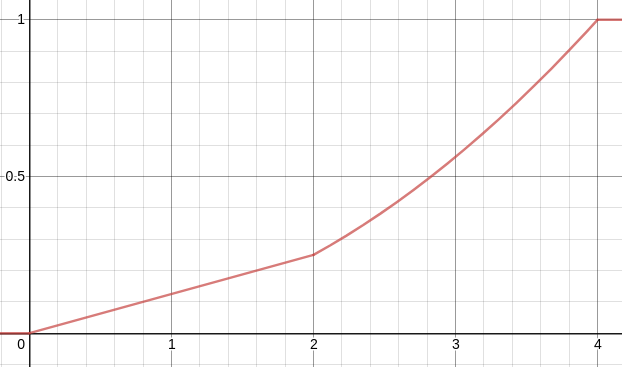
\includegraphics[scale=.6]{capture.png}\end{center}

    $X$ is a continuous random variable, since its CDF $F_X$ is continuous.
    
\newpage
\noindent{\bf c.}
    $$f_X(x) =
        \begin{cases}
            0 & x < 0, \\
            \frac18 & 0 \leq x < 2, \\
            \frac18x & 2 \leq x < 4, \\
            0 & x \geq 4.
        \end{cases}$$
        
    \begin{center}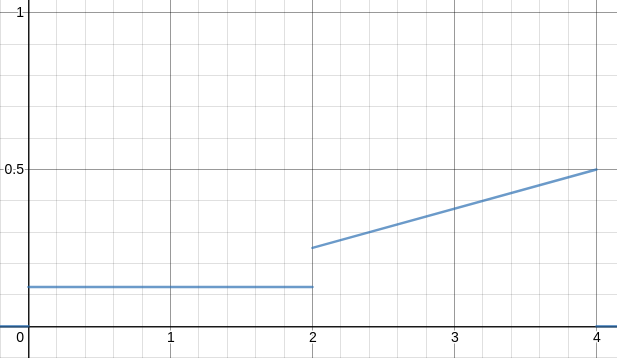
\includegraphics[scale=.6]{capture2.png}\end{center}
    
\medskip
\noindent{\bf d.}
\begin{align*}
    \mathbb P(1 < X < 3) &= F_X(3) - F_X(1) \\
                         &= \frac1{16} \cdot 3^2 - \frac18 \\
                         &= \frac7{16}.
\end{align*}

\medskip
\noindent{\bf e.}
\begin{align*}
    \mathbb P(X > 1~|~X<3) &= \frac{\mathbb P(1 < X < 3)}{\mathbb P(X < 3)} \\
                           &= \frac{F_X(3) - F_X(1)}{F_X(3)} \\
                           &= \frac{\frac7{16}}{\frac9{16}} \\
                           &= \frac79.
\end{align*}

\newpage
\noindent{\bf f.}
\begin{align*}
    \mathbb EX &= \int_{-\infty}^\infty f_X(x) \cdot x\,dx \\
               &= \int_{-\infty}^0 0x\,dx + \int_0^2 \frac18x\,dx + \int_2^4 \frac18x^2\,dx + \int_4^\infty 0x\,dx \\
               &= \int_0^2 \frac18x\,dx + \int_2^4 \frac18x^2\,dx \\
               &= \frac14 + \frac{4^3}{24} - \frac{2^3}{24} \\
               &= \frac{31}{12}
\end{align*}

\newpage
\noindent{\bf 2.}

\noindent{\bf a.} In statistics, a median is the value in a data set for which half of the data points are greater and half of the data points are less. This is sort of like the ``middle point" in the data set. Similarly, the median of a random variable is the value $m$ for which the probability that the variable is greater than $m$ is greater than $.5$, and the probability that the variable is less than $m$ is greater than $.5$. This is sort of like the ``middle point" of the possible values of the random variable.

\medskip
\noindent{\bf b.} Let $X\sim\text{Binomial}(1, .5)$. Then, $0$ and $1$ are both medians of $X$.

\medskip
\noindent{\bf c.}
\begin{proof}
    Let $X$ be a continuous random variable. Note that $\lim\limits_{x\to\infty} F_X(x) = 1$, and $\lim\limits_{x\to-\infty} F_X(x) = 0$. Thus, by the $(\epsilon, \delta)$ definition of a limit, there exist $c_1, c_2 \in \mathbb R$ such that $|F_X(c_1) - 0| < 0.1$ and $|F_X(c_2) - 1| < 0.1$. Since probabilities are between 0 and 1, we have that $F_X(c_1) < 0.1$ and $F_X(c_2) > 0.9$. Thus, since $F_X(x)$ is continuous, there exists $m$ such that $F_X(m) = 0.5$ by the intermediate value theorem. Thus, $\mathbb P(X \leq m) = 0.5 = 1 - \mathbb P(X \leq m) = \mathbb P(X \geq m)$, so $m$ is the median of $X$.
\end{proof}

\medskip
\noindent{\bf d.} We're looking for a real number $m$ such that
$$\mathbb P(X \geq m) \geq .5~\text{and}~\mathbb P(X \leq m) \geq .5.$$
We'll show later that the point at which the CDF crosses .5 satisfies this requirement.
\begin{align*}
    \frac1{16} x^2 &= \frac12 \\
    x^2 &= 8 \\
    x &= 2\sqrt2.
\end{align*}
Thus, the median of $X$ is $2\sqrt2$. This is greater than the mean of $X$.

\medskip
\noindent{\bf e.} Let $X$ be a real number chosen uniformly at random from $[0,1]$. Then, $\frac12 = \mathbb EX = m$, the median of $X$.

\newpage
\noindent{\bf 3.}
    $$f_Y(y) = \begin{cases}c(1-y^2) & -1 < y < 1, \\ 0 & \text{else.} \end{cases}$$

\noindent{\bf a.}
\begin{align*}
    \int_{-\infty}^{-1} 0\,dy + \int_{-1}^1 c(1-y^2) \, dy + \int_1^\infty 0\,dy &= 1 \\
    \int_{-1}^1 c(1-y^2) \, dy &= 1 \\
    \int_{-1}^1 (1-y^2) \, dy &=\frac1c \\
    \int_{-1}^1 1\,dy - \int_{-1}^1 y^2 \,dy &= \frac1c \\
    2 - (\frac{1^3}3 - \frac{(-1)^3}3) &= \frac1c \\
    \frac43 &= \frac1c \\
    \frac34 &= c
\end{align*}

\medskip
\noindent{\bf b.}
    \begin{center}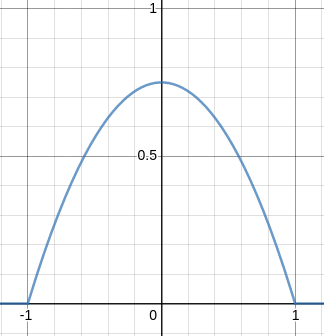
\includegraphics{capture3.png}\end{center}
    
\newpage
\noindent{\bf c.}
\begin{align*}
    F_Y(y) &= \int f_Y(y)\,dy \\
           &= \begin{cases} 0 & y \leq -1 \\ \frac14(3y-y^3) + \frac12 & -1 < y < 1 \\ 1 & y \geq 1\end{cases}
\end{align*}
(I added constants to these so that the CDF properties hold.)

\begin{center}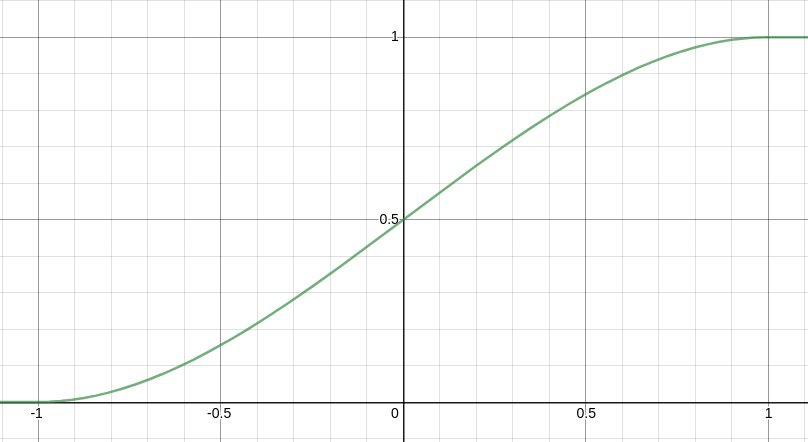
\includegraphics[scale=.5]{capture4.png}\end{center}

$Y$ is a continuous random variable because its CDF is continuous.

\medskip
\noindent{\bf d.}
\begin{align*}
    \mathbb P(0 < Y < 2) &= \mathbb P(0 \leq Y \leq 2) \\
                         &= F_Y(2) - F_Y(0) \\
                         &= 1 - \frac14(3\cdot0 - 0^3) + \frac12 \\
                         &= \frac12
\end{align*}

\medskip
\noindent{\bf e.} $$\mathbb P(Y = 0) = 0$$

\newpage
\noindent{\bf 4.} $$Z\sim{\text{Binomial}(3, .5)}$$
Then,
\begin{align*}
    F_Z(z) &= \sum_{i=0}^z \mathbb P(Z = i) \\
           &= \sum_{i=0}^z {3 \choose i}\left(\frac12\right)^i\left(\frac12\right)^{3-i} \\
           &= \sum_{i=0}^z {3 \choose i}\left(\frac{1}{2}\right)^{3} \\
           &= \frac18\sum_{i=0}^z {3 \choose i}
\end{align*}

\begin{center}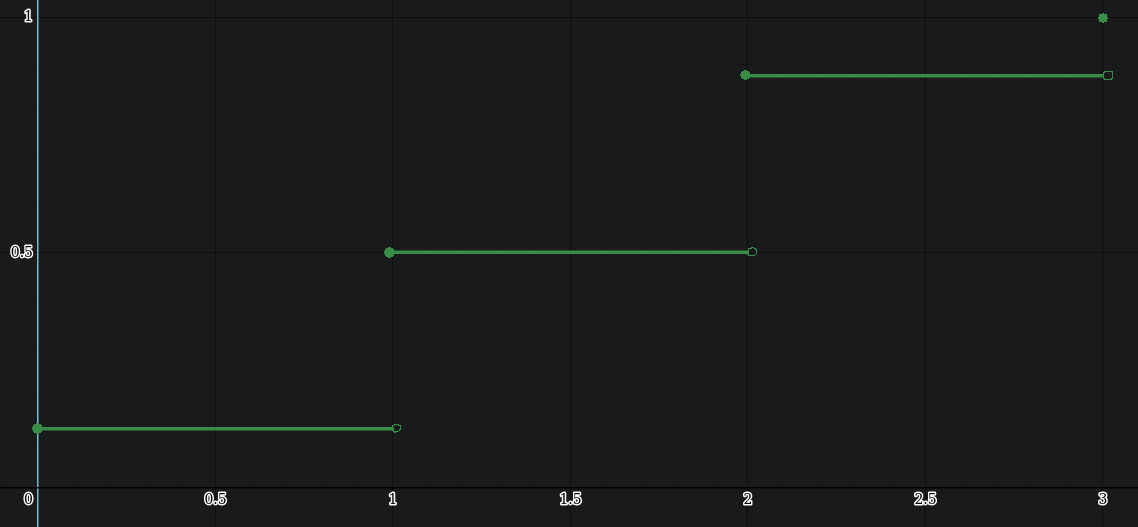
\includegraphics[scale=.5]{capture5.png}\end{center}

\end{document}
